\projecthead{04}{Rover structural analysis}{Frame design, load cases \& weight reduction}{September 2025 - present}
\textit{FEA lead / Stony Brook Robotics}
\par\medskip Design and analysis of the URC rover frame, using static and impact cases to guide structural changes before fabrication.
\par\smallskip {\small\color{muted} Tools: SolidWorks, Ansys Mechanical, LS-DYNA}
\medskip
\begin{center}
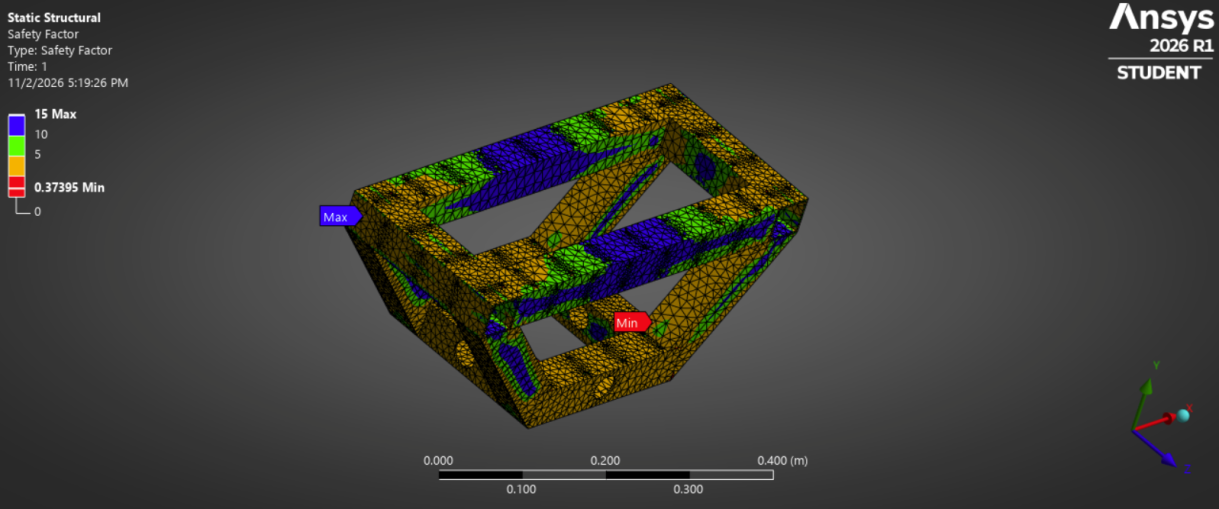
\includegraphics[width=\linewidth,height=2.5in,keepaspectratio]{images/rover/safety-factor-2026-11-02.png}
\par\smallskip{\footnotesize\color{muted} Static structural safety-factor plot (2 Nov 2026); displayed minimum 0.37395.}
\end{center}
\subsection*{My contribution}
I design the URC rover frame in SolidWorks and evaluate it in Ansys Mechanical. LS-DYNA supports short impact cases. Successive load-case iterations reduced the rover mass by 6 kg.
\subsection*{Top-frame study}
The September 2026 pass modeled aluminum 6061-T6 members with 5 mm joint connections. Loads of 100 N, 150 N, and 150 N were applied with selected faces fixed. This initial pass used the default mesh.
\subsection*{Design response}
Peak deformation on the middle member pointed to the layout as the area to improve. Proposed changes included additional supports, filleted trusses or L-bars, and evaluation of 2 x 2 inch tubing.